\documentclass{beamer}
\usepackage{beamerthemesplit}

%Definieren uns farbigen Quellcode
\usepackage{color}
\definecolor{dkgreen}{rgb}{0,0.6,0}
\definecolor{gray}{rgb}{0.5,0.5,0.5}
\definecolor{mauve}{rgb}{0.58,0,0.82}
 
%Damit wir Quellcode nutzen können.
\usepackage{listings}
\lstset{numbers=left,
	numberstyle=\tiny,
	numbersep=5pt,
	breaklines=true,
	showstringspaces=false,
	frame=l ,
	xleftmargin=15pt,
	xrightmargin=15pt,
	basicstyle=\ttfamily\scriptsize,
	stepnumber=1,
	keywordstyle=\color{blue},          % keyword style
  	commentstyle=\color{dkgreen},       % comment style
  	stringstyle=\color{mauve}         % string literal style
}
%Sprache Festelegen
\lstset{language=C++}

\begin{document}
\title{Infinite Impulse Response Filters} 
\author{Judith Massa, Patrick Esser}
\date{\today} 

\frame{\titlepage} 

\frame{\frametitle{Overview}\tableofcontents} 

\section{Motivation} 
\frame{\frametitle{ilastik} 
ilastik is a toolkit for interactive image classification and segmentation.
Sven Peter is working on object tracking.
Besides the image itself, algorithms rely on precomputed features of the
image.
}
\frame{\frametitle{Image Features} 
\begin{itemize}
  \item Scale-space representation
  \item Edges
  \item Corners
\end{itemize}
}

\frame{\frametitle{Gaussian Filtering} 
\begin{itemize}
  \item Convolution with Gaussian gives scale space representations
  \item Convolution with Gaussian derivative gives derivative of smoothed
    image (edge features)
\end{itemize}
Problem: Gaussian discretized to stencil. Coarse scale representation
corresponds to wide Gaussians - those need larger stencils, too!
}

\frame{\frametitle{Implementations of Filters}
\begin{itemize}
  \item Direct convolution
  \item FFT
  \item IIR
\end{itemize}
Notice that both direct convolution as well as FFT suffer from increasing
stencils and FFT does not always outperform direct convolution on GPUs.
\cite{1648322}
}


\section{IIR} 
\frame{\frametitle{The idea}
Instead of using the real, possibly wide stencil, approximate it by a fixed
size stencil. To compensate for reduced width of the stencil, use a
recursive filter.
}

\frame{\frametitle{The name}
Why infinite impulse response?
}

\frame{\frametitle{The consequences}
Approximation error - not too important here, we just use some
filters that we \emph{think} will produce useful features for subsequent
image analysis algorithms, so as long as it produces a visually
plausible result it should be acceptable.

Fixed computational cost - does not depend on scale parameter.

Less parallelism than FIR - each row's column depends on previous column's
result.
}

\begin{frame}[fragile]{The algorithm}
  \begin{lstlisting}
  int i = 42;
  \end{lstlisting}
\end{frame}


\section{Parallelization}
\frame{\frametitle{Possibilities and challenges}
\begin{enumerate}
  \item All rows independent
  \item Causal and anticausal pass independent
  \item Vertical pass causes bad memory layout
  \item Parallelize recurrence relation within each row
\end{enumerate}
}

\frame{\frametitle{Prioritize}
Keep in mind: Different data and applications need different optimizations.
Our data: Image sequences of approximately 1024x1024 pixels.
\begin{itemize}
  \item Rows consist of approximately 1000 elements so it must be evaluated
    whether a (more complicated) parallelization of the recurrence relation
    within rows pays off. \cite{blelloch1990prefix}
\end{itemize}
}

\frame{\frametitle{Hiding data transfers}
\begin{itemize}
  \item Usually multiple features (around 10) are calculated for each image,
    thus we only have to transfer an image once to the device and we can
    interleave device to host transfers with outstanding feature
    calculations without requiring a modification of the algorithm.
  \item Similiarly, since we are working on independent sequences of images
    we can hide host to device transfers. Thus we consider the
    parallelization of the algorithm orthogonal to hiding data transfers (in
    contrast to, e.g. trying to start computations on rows of the image as
    soon as they arrive to hide latencies \emph{within a single}
    image - instead we hide transfers \emph{between multiple} images.
\end{itemize}
}

\begin{frame}{For each parallelization}
  \begin{figure}
    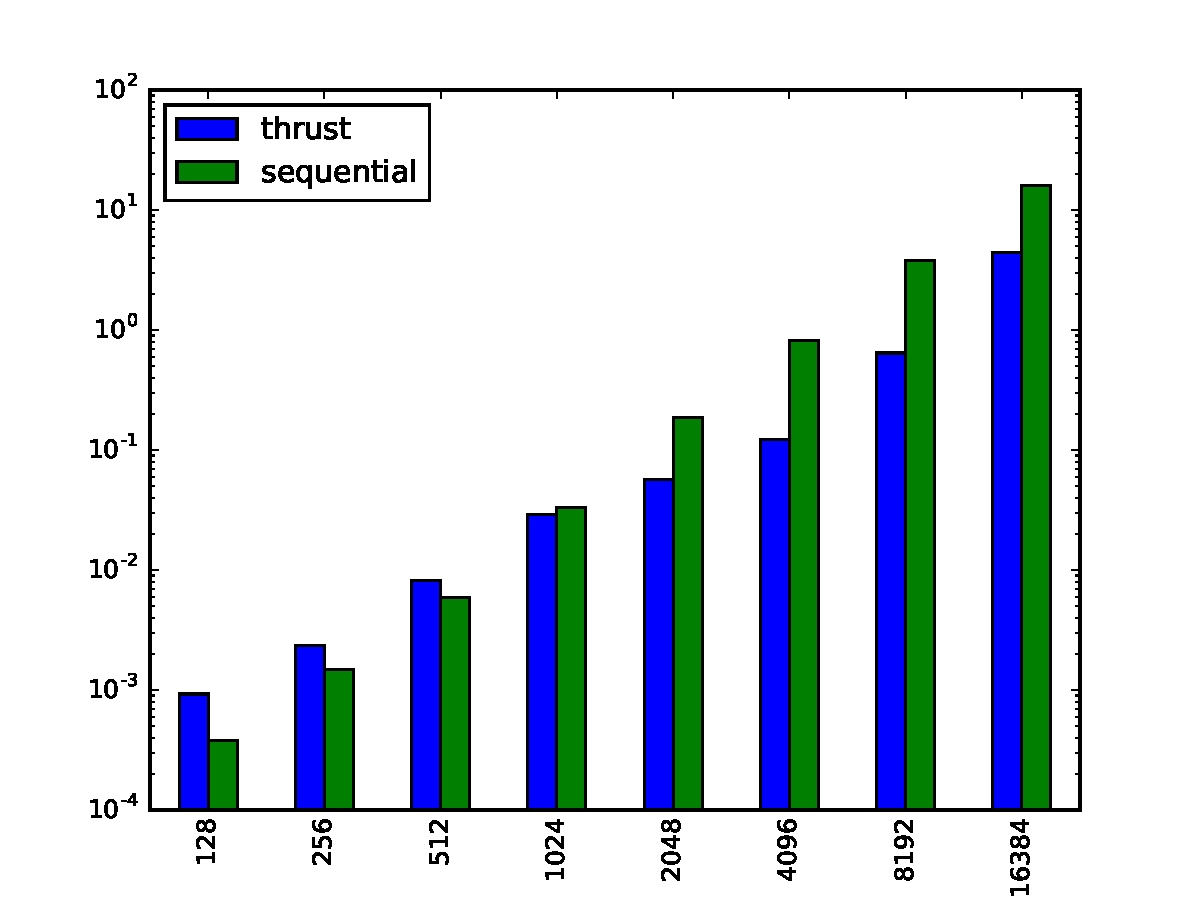
\includegraphics[scale=0.4]{imgs/thrust_vs_sequential_total.pdf} 
  \end{figure}
\end{frame} 

\begin{frame}{A closer look}
  \begin{figure}
    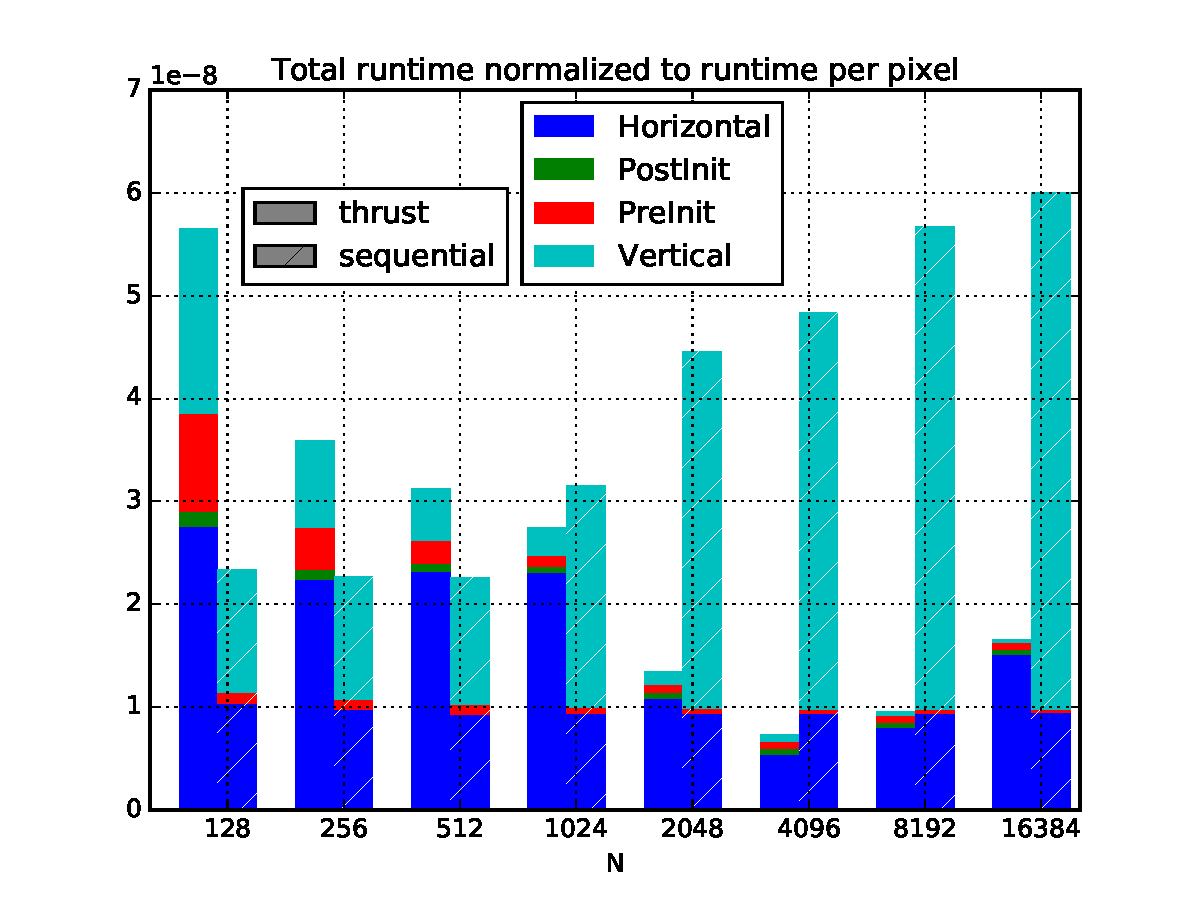
\includegraphics[scale=0.4]{imgs/thrust_vs_sequential_normalized.pdf} 
  \end{figure}
\end{frame} 


\section{Conclusion} 
\frame{\frametitle{Conclusion}
ToDo: Compare to FIR and FFT.
Explore blocked parallelism.
Hide data transfers.
}

%\begin{frame}[t, allowframebreaks]
\begin{frame}[t]
  \frametitle{References}
  \bibliographystyle{amsalpha}
  \bibliography{doc.bib}
\end{frame}

\end{document}
